\def\mySecNum{3.4}
\mySection{\mySecNum~Speculating on volatility}
%-------------- start slide -------------------------------% {{{
\begin{frame}[fragile,t]
	\begin{center}

		\begin{minipage}{0.37\textwidth}
			\textcolor{magenta}{Directional positions}
			\pause
			\begin{itemize}
				\item Bull spread
				\item Bear spread
				\item Collars
				\item Box spreads
			\end{itemize}
		\end{minipage}

		\pause
		\bigskip
		\mySeparateLine
		\bigskip

		\begin{minipage}{0.37\textwidth}
			\textcolor{cyan}{Nondirectional positions}
			\pause
			\begin{itemize}
				\item Straddles
				\item Strangle
				\item Butterfly spread
			\end{itemize}
		\end{minipage}
		\bigskip

		\pause
		Investors who do not care whether the stock goes up or down, \\
		but only \alert{how much it moves}.                          \\
		\bigskip

		Investors are speculating on                                 \\
		\bigskip

		\alert{\huge volatility}
	\end{center}
\end{frame}
%-------------- end slide -------------------------------%}}}
%-------------- start slide -------------------------------%{{{ 1
\begin{frame}[fragile,t]
	\frametitle{Example for this section}
	\begin{center}
		Black-Scholes option prices \\
		\begin{align*}
			\text{Stock price}                     & = \$40   \\
			\text{Volatility}                      & = 30\%   \\
			\text{Effective annual risk-free rate} & = 8.33\% \\
			\text{Dividend yield} & = \$0 \\
			\text{Expriation days} & = 91~\text{days}
		\end{align*}

		\bigskip
		\renewcommand{\arraystretch}{1.2}
		\begin{tabular}{ccc}
			\hline
			Strike & Call & Put  \\
			\hline
			35     & 6.13 & 0.44 \\
			40     & 2.78 & 1.99 \\
			45     & 0.97 & 5.08 \\
		\end{tabular}
		\end{center}
\end{frame}
%-------------- end slide -------------------------------%}}}
%-------------- start slide -------------------------------%{{{ 1
\begin{frame}[fragile,t]
	\frametitle{Straddles}

	\textcolor{magenta}{\bf Straddle} is the strategy of buying a call and a put with the same strike
	price and time to expiration.
	\bigskip

	A straddle is a bet that \textcolor{red}{volatility will be high} relative to the market’s assessment
	\bigskip

	\begin{center}
		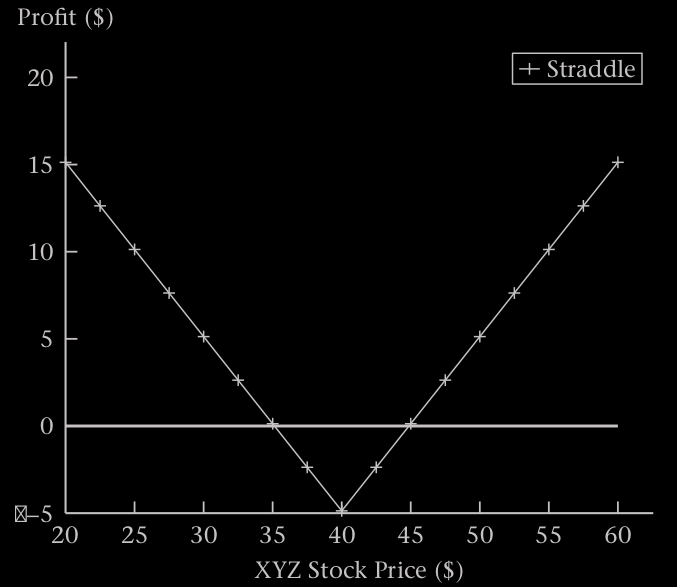
\includegraphics[scale=0.25]{figs/Figure-3-10.png}
	\end{center}
\end{frame}
%-------------- end slide -------------------------------%}}}
%-------------- start slide -------------------------------%{{{ 1
\begin{frame}[fragile,t]
\begin{myexample}
	Draw the profit graph for a \$40=strike straddle.
\end{myexample}
\pause
\bigskip
\begin{mysol}
	We only need to determine the tip of the graph:
	\begin{align*}
		-(2.78+1.99) \times (1+0.083)^{1/4} = -\$ 4.8660.
	\end{align*}
	Hence,

	\begin{center}
		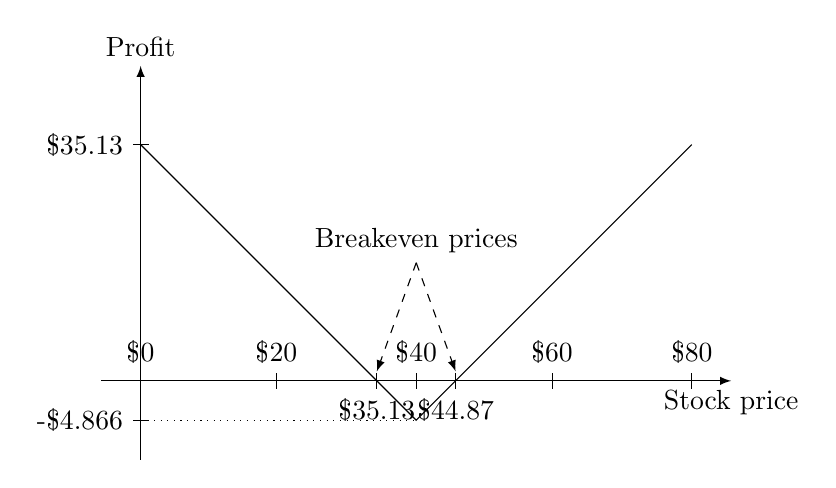
\begin{tikzpicture}[scale=1, transform shape]
			\tikzset{>=latex}
			\draw[->] (-0.5,0) -- (7.5,0) node [below] {Stock price};
			\draw[->] (0,-1) -- (0,0.1) node [above] {\$0} -- (0,4) node [above] {Profit};
			\draw (0,3) -- (3.5,-0.5) -- (7,3);
			\draw (0.1,-0.5) -- ++(-0.2,0) node [left] {-\$4.866};
			\draw (3,0.1) -- ++(0,-0.2) node [below] {\$35.13};
			\draw (4,0.1) -- ++(0,-0.2) node [below] {\$44.87};
			\draw (3.5,-0.1) -- ++(0,0.2) node [above] {\$40};
			\draw (1.725,-0.1) -- ++(0,0.2) node [above] {\$20};
			\draw (5.225,-0.1) -- ++(0,0.2) node [above] {\$60};
			\draw (7,-0.1) -- ++(0,0.2) node [above] {\$80};
			\draw (0.1,3) -- ++(-0.2,0) node [left] {\$35.13};
			\draw [dashed, ->] (3.5,1.5) node[above] {Breakeven prices} -- (3,0.12);
			\draw [dashed, ->] (3.5,1.5) -- (4,0.12);
			\draw [dotted] (0,-0.5) -- ++(3.5,0);
		\end{tikzpicture}
	\end{center}
	\myEnd
\end{mysol}
\end{frame}
%-------------- end slide -------------------------------%}}}
%-------------- start slide -------------------------------%{{{ 1
\begin{frame}[fragile,t]
	\frametitle{Strangle}

	\textcolor{cyan}{\bf Strangle} is the strategy of	buying an out-of-the-money call and put with
	the same time to expiration.
	\bigskip

	\begin{center}
		A \textcolor{cyan}{strangle} can be used to reduce the high premium cost, \\
		associated with a \textcolor{magenta}{straddle}.
	\end{center}

	\vfill
	\begin{center}
		\renewcommand{\arraystretch}{1.2}
		\begin{tabular}{c|cc}
			\hline
                                    & Buying call at a strike price & Buying put at a strike price \\ \hline
			\textcolor{magenta}{Straddle} & Same                          & Same                         \\
			\textcolor{cyan}{Strangle}    & High                          & Low                          \\
			\hline
		\end{tabular}

	\end{center}
\end{frame}
%-------------- end slide -------------------------------%}}}
%-------------- start slide -------------------------------%{{{ 1
\begin{frame}[fragile,t]
	\begin{myexample}
		Draw profit diagram for 40-strike straddle and strangle composed of
		\begin{align*}
			\text{35-strike put} + \text{45-strike call}.
		\end{align*}
	\end{myexample}
	\pause
	\bigskip
	\begin{mysol}
		We know the shape of the graph and need only to determine the level of the flat part. Hence,
		suppose the stock price is \$40. Then the profit is
		\begin{align*}
			-(0.44+0.97)\times(1+0.083)^{1/4}=-\$1.4384.
		\end{align*}
		The breakeven prices are
		\begin{align*}
			45+1.4384 = \$46.4384 \quad \text{and} \quad 35-1.4384 = \$ 33.562.
		\end{align*}
	\end{mysol}
\end{frame}
%-------------- end slide -------------------------------%}}}
%-------------- start slide -------------------------------%{{{ 1
\begin{frame}[fragile,t]
	\begin{center}
		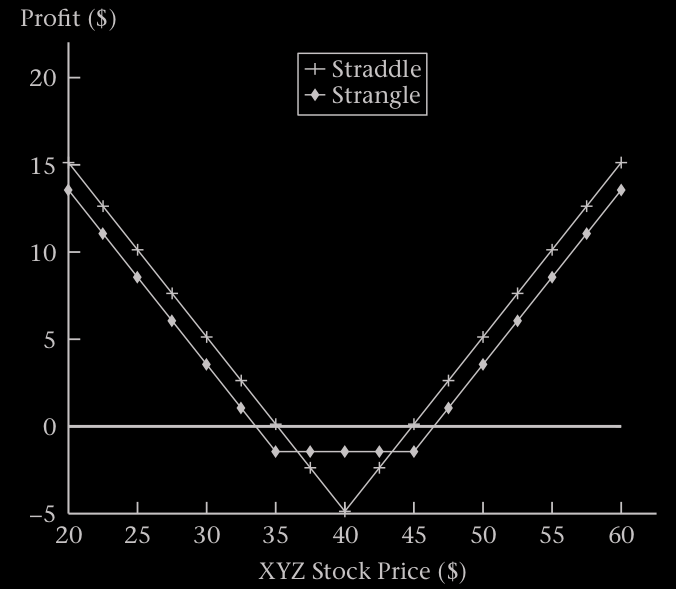
\includegraphics[scale=0.25]{figs/Figure-3-11.png}
	\end{center}
	\myEnd
\end{frame}
%-------------- end slide -------------------------------%}}}
%-------------- start slide -------------------------------% {{{
\begin{frame}[fragile,t]
	\frametitle{Written straddles}

	\textcolor{magenta}{\bf Written straddle} is the strategy of
	selling a call and put with the same strike price and time to maturity.
	\bigskip


	\begin{center}
		Unlike a purchased straddle, a written straddle is a bet that \\
		\bigskip

		\textcolor{red}{volatility will be low}
		\bigskip

		relative to the market’s assessment.
	\end{center}

	\bigskip

	\begin{center}
		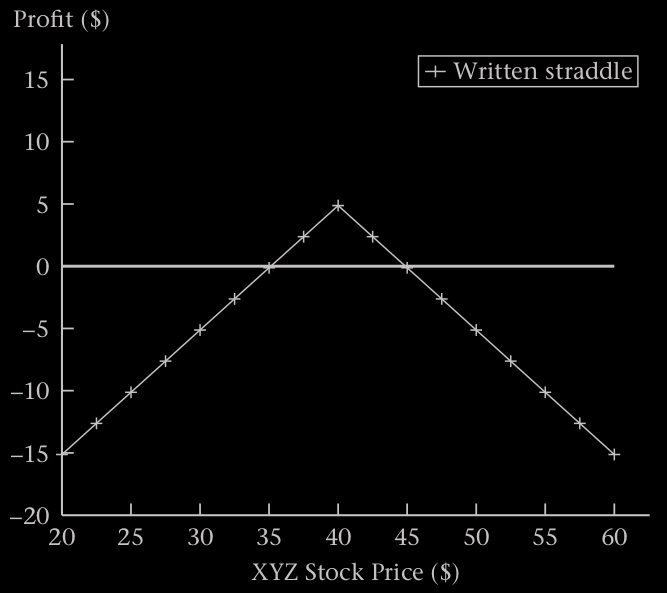
\includegraphics[scale=0.25]{figs/Figure-3-12.png}
	\end{center}
\end{frame}
%-------------- end slide -------------------------------%}}}
%-------------- start slide -------------------------------% {{{
\begin{frame}[fragile,t]
	\frametitle{Butterfly spreads}
	\begin{align*}
		\text{\textcolor{magenta}{\bf Butterfly spreads}} & = \text{Insured wri\text{en straddle}} \\
																											& = \text{\textcolor{magenta}{Written straddle}}  + \text{\textcolor{cyan}{purchased straggle}}
	\end{align*}

	\begin{center}
		A butterfly spread insures against large losses on a straddle.
		\bigskip
		\bigskip

		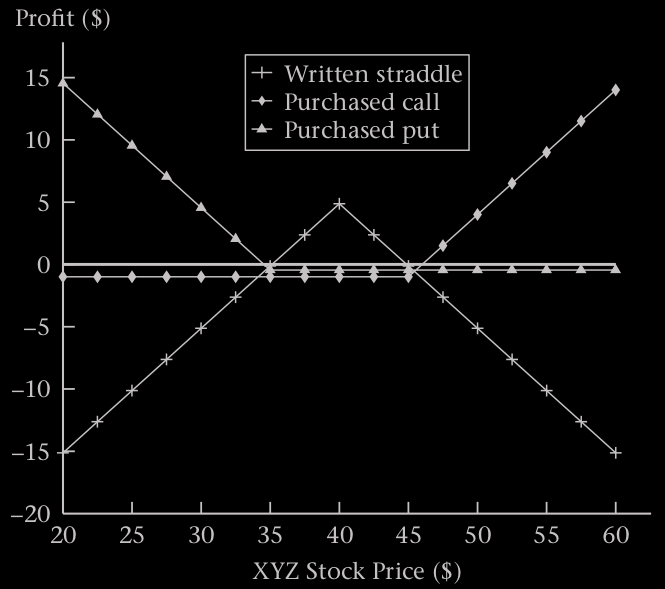
\includegraphics[scale=0.2]{figs/Figure-3-13.png}
		\quad
		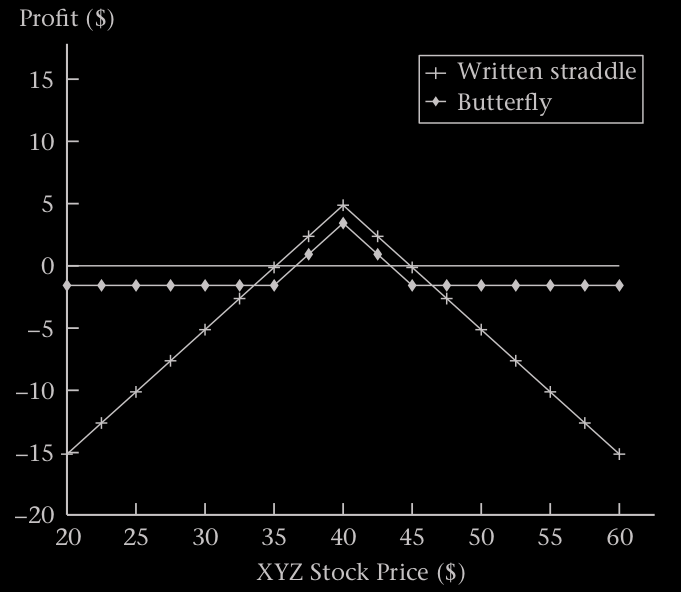
\includegraphics[scale=0.2]{figs/Figure-3-14.png}
	\end{center}
\end{frame}
%-------------- end slide -------------------------------%}}}
%-------------- start slide -------------------------------%{{{ 1
\begin{frame}[fragile,t]
\begin{myexample}
	Draw the profit graph for the butterfly spread:
	\begin{align*}
		\text{Written \$40 \textcolor{magenta}{straddle}} + \text{purchased 35-45 \textcolor{cyan}{straggle}}.
	\end{align*}
	\pause \bigskip

	\begin{mysol}
		First notice that this spread corresponds:
		\begin{center}
			\renewcommand{\arraystretch}{1.2}
			\begin{tabular}{ccc}
				\hline
				Strike & Call                              & Put                               \\
				\hline
				35     & 6.13                              & 0.44 (\textcolor{cyan}{long})     \\
				40     & 2.78 (\textcolor{magenta}{short}) & 1.99 (\textcolor{magenta}{short}) \\
				45     & 0.97 (\textcolor{cyan}{long})     & 5.08                              \\
			\end{tabular}
		\end{center}
		We know the general shape of the profit graph and need only to determine the level when the graph is flat. For this, suppose that the stock price is \$ $x<30$.
		In this case, only both puts are in the money and the profit is
		\begin{align*}
			(\textcolor{magenta}{2.78}+\textcolor{magenta}{1.99} - \textcolor{cyan}{0.44} -\textcolor{cyan}{0.97}) \times (1+0.083)^{1/4} + (35-x) + (x-40) = -\$1.5724.
		\end{align*}
	\end{mysol}
	% (2.78+1.99-0.44-0.97)*(1.083^0.25) -5
\end{myexample}
\end{frame}
%-------------- end slide -------------------------------%}}}
%-------------- start slide -------------------------------%{{{ 1
\begin{frame}[fragile,t]
	\begin{center}
			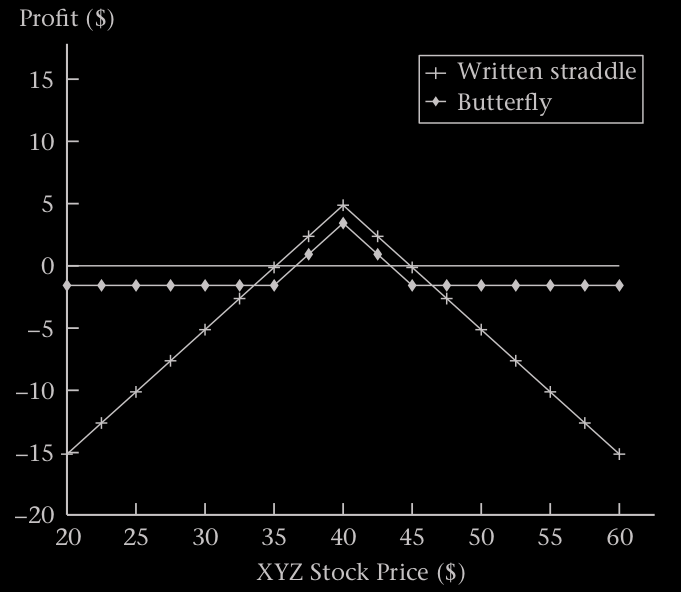
\includegraphics[scale=0.3]{figs/Figure-3-14.png}
	\end{center}
	\myEnd
\end{frame}
%-------------- end slide -------------------------------%}}}
